\IfFileExists{tables/frontend_adaptation.tex}{%
Lightweight adaptation restores the benefit on every front end. Table~\ref{tab:frontend_adaptation} reports the complete \(8\times4\) matrix in which the frozen reference checkpoint and seven adapted models are each evaluated on all four front ends; Supplementary Fig.~\ref{S-fig:frontend_adaptation} visualizes the corresponding relative recovery. Each adaptation updates either the gate and residual heads only or all parameters for 20 epochs on training and validation actions, without test data. Full target-specific adaptation reduces the matched-front-end error to 0.2290 for VideoPose3D, 0.2741 for PoseFormer, and 0.2393 for MotionBERT, which is 52.0\%, 39.7\%, and 49.8\% below the canonical average of the respective front end (0.4776, 0.4542, and 0.4766) and 57.5\%, 48.9\%, and 45.4\% below the frozen checkpoint on the same input. A single model adapted on a balanced mixture of all four front ends reaches 0.2363, 0.2751, and 0.2464 on the three alternatives while retaining 0.1809 on SAM3D, which is 16.7\% above the native checkpoint but still 35.2\% below canonical averaging. Thus one architecture, adapted with a short schedule, improves over canonical averaging on every tested front end; the remaining trade-off is between recovery on the target front end and retention on the native one, since no adapted model dominates the frozen checkpoint on every input source.
\begin{table*}[t]
\centering
\caption{Common-13 MPJPE after front-end-specific or mixed adaptation. Each row is one frozen model evaluated on all four front ends; lower is better.}
\label{tab:frontend_adaptation}
\small
\begin{tabular}{lrrrr}
\toprule
Adaptation model & SAM3D & VideoPose3D & PoseFormer & MotionBERT \\
\midrule
Frozen reference & 0.1551 & 0.5389 & 0.5360 & 0.4385 \\
\midrule
VideoPose3D/heads & 0.2120 & 0.2621 & 0.3297 & 0.3567 \\
VideoPose3D/full & 0.2442 & 0.2290 & 0.2954 & 0.4403 \\
PoseFormer/heads & 0.1822 & 0.2833 & 0.3234 & 0.3521 \\
PoseFormer/full & 0.2033 & 0.2447 & 0.2741 & 0.3381 \\
MotionBERT/heads & 0.1976 & 0.4667 & 0.5100 & 0.2744 \\
MotionBERT/full & 0.2117 & 0.5050 & 0.6036 & 0.2393 \\
Mixed/full & 0.1809 & 0.2363 & 0.2751 & 0.2464 \\
\bottomrule
\end{tabular}
\end{table*}


}{%
\paragraph{Pending result} Front-end adaptation results will be inserted only after all seven training runs and all 32 test cells pass the no-leakage and full-split validators.
}

\FloatBarrier
\subsection{Scaling beyond two views}

\IfFileExists{tables/nview_scaling.tex}{%
Figure~\ref{fig:nview_scaling} shows accuracy and bootstrap intervals under frozen pairwise composition, while Table~\ref{tab:nview_efficiency} reports its computational cost. Supplementary Table~\ref{S-tab:nview_scaling} provides the numerical means, standard deviations, and intervals for all methods. Accepted and rejected camera groups are retained in the runtime manifest so that missing common frames are not silently converted into favorable subsets.
\begin{table}[t]
\centering
\caption{Accuracy--cost trade-off for deployable frozen pairwise composition. Latency is the serial fusion time per 30-frame camera group; reduction is relative to the two-view MPJPE.}
\label{tab:nview_efficiency}
\footnotesize
\setlength{\tabcolsep}{4pt}
\begin{tabular}{@{}rrrrrrrr@{}}
\toprule
Views & Pairs & MPJPE & Red. (\%) & Latency (ms) & Rel. & Groups/s & Peak MiB \\
\midrule
2 & 1 & 0.1295 & -- & 2.02 & 1.00$\times$ & 494.7 & 12.28 \\
3 & 3 & 0.1177 & 9.1 & 6.02 & 2.98$\times$ & 166.1 & 12.31 \\
4 & 6 & 0.1158 & 10.6 & 12.06 & 5.96$\times$ & 83.0 & 12.33 \\
\bottomrule
\end{tabular}
\vspace{0.3em}
\begin{minipage}{0.97\linewidth}\footnotesize Serial latency is the synchronized mean over 44 accepted 30-frame camera groups after 10 warm-up executions on one NVIDIA RTX A6000. It includes pose canonicalization, all unique pair forwards, and output averaging, but excludes monocular front-end inference, data loading, and oracle selection.\end{minipage}
\end{table}

A separate matched local-model audit (Supplementary Section~\ref{S-sec:local_fusion_efficiency}) measures parameter size, matrix/convolution operation counts, and fusion latency for CanonFuse3D, the local TCN, and SmoothNet. CanonFuse3D has 235,524 parameters but higher latency than these two temporal baselines; its purpose is cross-view refinement rather than minimum-cost smoothing. This audit excludes upstream inference and uses a narrower timing boundary than the serial N-view measurements.
The method-specific external audit (Supplementary Table~\ref{S-tab:external_fusion_efficiency}) measures STRIDE~\cite{lal2025stride}, DeciWatch~\cite{zeng2022deciwatch}, and MetaPose~\cite{usman2022metapose} on the same GPU. Their adapted 30-frame paths take 755.513~ms including STRIDE's 30 test-time updates, 3.123~ms for DeciWatch's sparse recovery, and 18.927~ms including MetaPose's initialization and coordinate adapters. STRIDE's final inference alone takes 12.095~ms and must not be substituted for its full adaptation cost. MetaPose retains its FP64 learned solver. Input joints, host transfers, and computational contracts differ, so these values describe deployment costs rather than a matched-input speed ranking; none includes the RGB front end.
The two-view configuration captures the largest gain: it reduces MPJPE from the single-view value of 0.1715 to 0.1295 (24.5\%) with one pair forward and 2.02~ms serial fusion latency. Three views reduce MPJPE by a further 9.1\% relative to two views, but require three pair forwards and 6.02~ms (2.98-fold) latency. Four views reach 0.1158 MPJPE, a 10.6\% reduction relative to two views, while requiring six pair forwards and 12.06~ms (5.96-fold) latency; the incremental gain from three to four views is only 1.6\%. Thus, additional views remain useful when accuracy is prioritized, whereas two views provide the most favorable accuracy--cost operating point for the main CanonFuse3D configuration.
\begin{figure}[!htb]
\centering
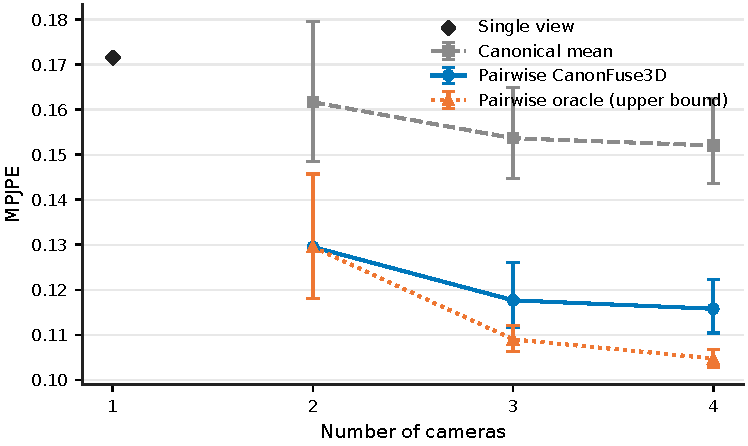
\includegraphics[width=0.72\linewidth]{figures/extension/nview_scaling.pdf}
\caption{N-view scaling under frozen pairwise CanonFuse3D composition. Error bars show paired-group bootstrap 95\% confidence intervals. The oracle is an upper bound.}
\label{fig:nview_scaling}
\end{figure}
}{%
\paragraph{Pending result} The N-view table and figure will be inserted only after the strict common-frame filter and the complete N=1--4 result matrix pass the artifact validator.
}

\FloatBarrier
\subsection{Automatic synchronization diagnostic}

\IfFileExists{tables/temporal_alignment.tex}{%
Figure~\ref{fig:temporal_alignment} compares uncorrected, automatically corrected, and oracle streams across the eleven injected offsets. Supplementary Table~\ref{S-tab:temporal_alignment} reports the exact errors together with lag-estimation accuracy and correction-activation rates. The confidence threshold (0.09296) was fixed from validation data before these test results were read. The result is directionally asymmetric. Automatic correction improves MPJPE for every tested positive lag: at \(+5\) frames, it reduces error from 0.1537 to 0.1506, versus the 0.1488 oracle. It also gives smaller improvements at \(\pm0.5\) frames. In contrast, it worsens every tested negative integer lead; at \(-5\) frames, error increases from 0.1484 to 0.1498. At zero offset, 41.5\% of samples activate a nonzero correction and MPJPE increases slightly from 0.14879 to 0.14884. Exact lag accuracy is only 13.2\% at \(+5\) frames. Thus, the descriptor is a useful diagnostic and partially recovers positive delays, but it is not a reliable bidirectional synchronization solution. We do not use it to strengthen the main CanonFuse3D comparison.
\begin{figure}[!htb]
\centering
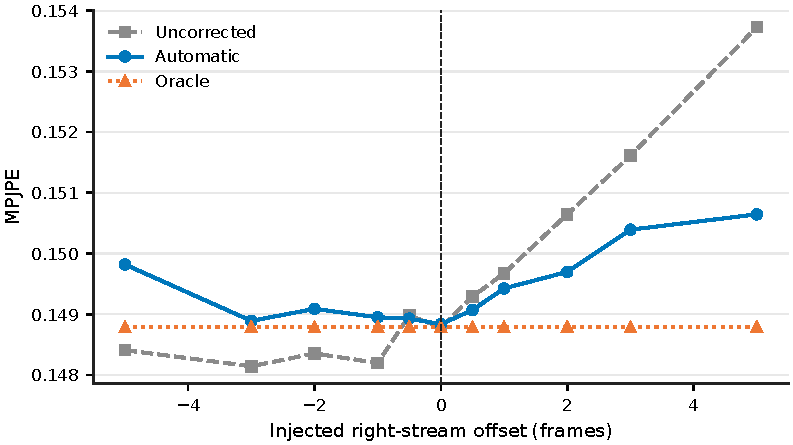
\includegraphics[width=0.72\linewidth]{figures/extension/temporal_alignment.pdf}
\caption{MPJPE under injected right-stream offsets on the fixed central 20-frame interval. Oracle restores the original unperturbed right stream; automatic correction uses the validation-calibrated confidence threshold.}
\label{fig:temporal_alignment}
\end{figure}
}{%
\paragraph{Pending result} Temporal-alignment results will be inserted only after all 33 offset-condition cells and the validation-threshold provenance pass validation.
}
